\section{Aplicación de ejemplo}
(Fijarse si se puede poner en la problemática)\\
1)Edición con cancelar\\
2)múltiple cancelaciones\\
3)buscador\\
4)monitor de transacciones\\

Para comprender mejor esta problemática veamos un ejemplo. Supongamos una simple
aplicación de banca donde los clientes de un banco pueden consultar el estado de sus
cuentas, realizar transferencias de fondos y administrar sus datos personales.
Al realizar un transferencia, desde una cuenta hacia otra, hay que extraer el
monto indicado de la primera cuenta, y depositarlo en la segunda. Estas dos
operaciones pueden tener errores, como por ejemplo, extraer un monto mayor al
saldo, o depositar mas cantidad de la maxima permitida.

		\begin{figure}[h]
			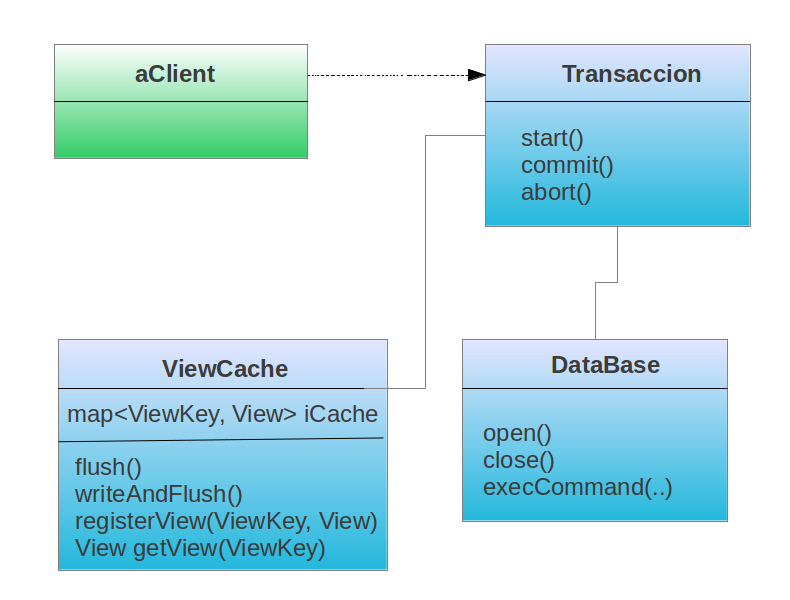
\includegraphics{img/objectTransaction}
			\caption{uml}
			\label{uml}
		\end{figure}	
	



\section{Nuestra herramienta: }

Con el propósito de cumplir el objetivo detallado en la Sección
\ref{sec:Objetivo} y llevándolo a cabo con la solución propuesta en la  la
Sección \ref{sec:Solucion}, se desarrolló una herramienta que llamamos
\emph{Aspect for Pure Object }.

\bigskip 

\emph{ Aspect for Pure Object} \emph{APO} es una abstracción del Framework
Javassist, que nos permite fácilmente implementar un aspecto, y aplicarlo a un grupo de
objetos.

\bigskip 

Se evaluaron dos frameworks para resolver nuestro problema. Uno es Javassist y
el otro AspectJ. \cite{KiczalesHHKPG01}

\bigskip

Se utiliza Javassist porque es independiente al usuario, en cambio si utilizamos
AspectJ obligamos al usuario a cambiar la implementación de sus objetos,
y cambiar el compilador del código. 

\bigskip

Utilizando esta herramienta se implementaron dos aspectos diferentes:

	\subsection{Aspecto Transaccional:} Esta basado en una implementación
	hecha por Nicolás Passerini y Javier Fernandes.
	 
	Utilizando la programación orientada a aspectos, intercepta todas las lecturas
	y escrituras de los fields. Insertando código al momento de la carga de la 
	clase.
	Se remplaza el acceso al field, tanto de lectura como escritura, y se lo delega
	al ObjectTransactionManager, donde se guarda la información en una estructura
	[objeto, [Field, Valor]].
	
	\bigskip
	
	El contexto esta asociado a un solo tread, implementado con varíales del tipo
	ThreadLocal. Esto me permite manejar la concurrencia en el acceso a la
	información de los objetos. Soporta transacciones anidadas, donde cada
	transacción hija hereda el estado de su padre, y al momento de hacer un commit
	en la sub-transacción, su cambios son impactados en la transacción padre.
	Por esta forma de implementación, la identidad del objeto se mantiene, ya que
	el objeto no se modifica ni se clona, solo se cambia el acceso a sus fields.

	\subsection{ Aspecto Observable}
			
	En su implementación interna lo que hace el aspecto es agregar un field del
	tipo \emph{PropertyChangeSupport} al objeto que se va a convertir en
	Observable. Y a su vez le agrega métodos para completar su objetivo.
	El primero es el \emph{firePropertyChange} que es el que notifica a los
	Observadores que una propiedad ha cambiado.	Luego le agregamos
	\emph{addPropertyChangeListener} y \emph{removePropertyChangeListener} para
	poder agregar y remover Observadores para que escuchen sus cambios.


\subsection{Integración con el dominio } 
	La integración con el dominio es fácil, se puede configurar con
	anotaciones, y el Framework me permite poder tener uno u otro aspecto, o
	ambos.
	
	{ponemos código de ejemplo????}
	
	\begin{lstlisting} 
		@TransactionalAndObservable
		public class Socio extends Entity {
		}
	\end{lstlisting}
	
	
	
\subsection{Integración de aspectos con el Arena}
En Arena se integró los dos aspectos, el Observable y el transaccional, con el
fin de que los objetos de dominio sean puros, y que no tengan la noción de
eventos, ni transacciones, y así poder bindearlos con los componentes de de la
interfaz gráfica. Y al cancelar la edición poder revertir los cambios
transparéntenme.

Para ello se tubo que asociar una transacción con una ventana, en el caso mas
especifico con la clase \emph{TransactionalDialog}. A su vez también tenemos
vinculado los eventos del dominio junto con la ventana y la transacción.
Se implemento tres niveles de aislamiento de los eventos,  \emph{Fire All},
\emph{Fire Committed} y \emph{Fire olnly in my transaction};

\begin{description}
	\item[\emph{Fire All}] Todos los eventos disparados por el dominio son
	escuchados, sin importar si están en una transacción.

	\item[\emph{Fire Committed}] Solo se escucha los eventos de las transacciones
		comiteadas
	
	\item[\emph{Fire olnly in my transaction}] solo se escucha los eventos que
		ocurren dentro de su translación.

 \end{description}
(Ver como redactar mejor esto\ldots ).

	
\subsection{Buscar un  titulo}
La implementación de la integración en el arena se realizó con Scala, agregando
mejora al Arena como: Árboles, Listas \ldots \ldots \ldots. 
	
	
Contar que esta publicado, con la licencia y blah

Test de los aspectos


